\chapter{Song-Havlin-Makse self-similar model}

\resp{Franco Aquistapace Tagua}

\section{Introduction and methods}
 
The work by Song, Havlin and Makse \cite{song2006origins} aims to explain the characteristic features of empirical scale--free fractal and non--fractal networks by means of a single growth model, that has the concept of renormalisation at its core. More specifically, the proposed growth mechanism works as the inverse of the renormalisation procedure. The goal of this task is then to reproduce their growth and renormalisation procedures, and to recover the characteristic behaviour of fractal and non--fractal networks through relevant descriptors.

The renormalisation of a network was done as described in the source material, by covering its $N$ nodes with $N_B(L_B)$ boxes, where the maximum shortest path between any two nodes in a box must be $L_B$. This is done algorithmically as follows:

\begin{enumerate}
	\item Initialise a box with a randomly picked node.
	\item For every remaining node $i$, add it to the box if $\max_{j\in B} d(i,j) \leq L_B$, where $B$ contains the nodes currently in the box, and $d(i,j)$ is the shortest path between nodes $i$ and $j$.
	\item Repeat steps 1. and 2. with the remaining available nodes until all nodes are assigned to a box.
\end{enumerate}

On the opposite hand, when performing the growth process of a network, each existing node is considered as a future hub. For a node with degree $k$, $mk$ offspring nodes are attached to it at each growth step. Then, each edge between two of the original nodes is removed with probability $p=1-e$, and replaced by an edge between two of their offspring. Thus, parameter $e$ represents hub--hub attraction / repulsion, with $e\rightarrow1$ being hub--hub attraction, and $e\rightarrow0$ being hub--hub repulsion. This growth process is referred to as the minimal model.

For each case in $e=1.0, 0.8$, a set of 10 graphs is generated with the minimal model. In all cases, the network is initialised as a star graph with $N_{init}=5$ nodes. Then, the growth mechanism is applied $n_{growth}=4$ times, with a growth factor of $m=2$. Once obtained, each graph is then subjected to the normalisation procedure with distances $1\leq L_B\leq32$. Furthermore, for each minimal model graph an uncorrelated version is generated by random swapping of links, while maintaining the degree distribution. The normalisation procedure is also applied to the randomised graphs. The specific details of the methodology can be found in the Supplementary Material.



\section{Results and discussion}


\begin{figure}[!h]
	\begin{center}
	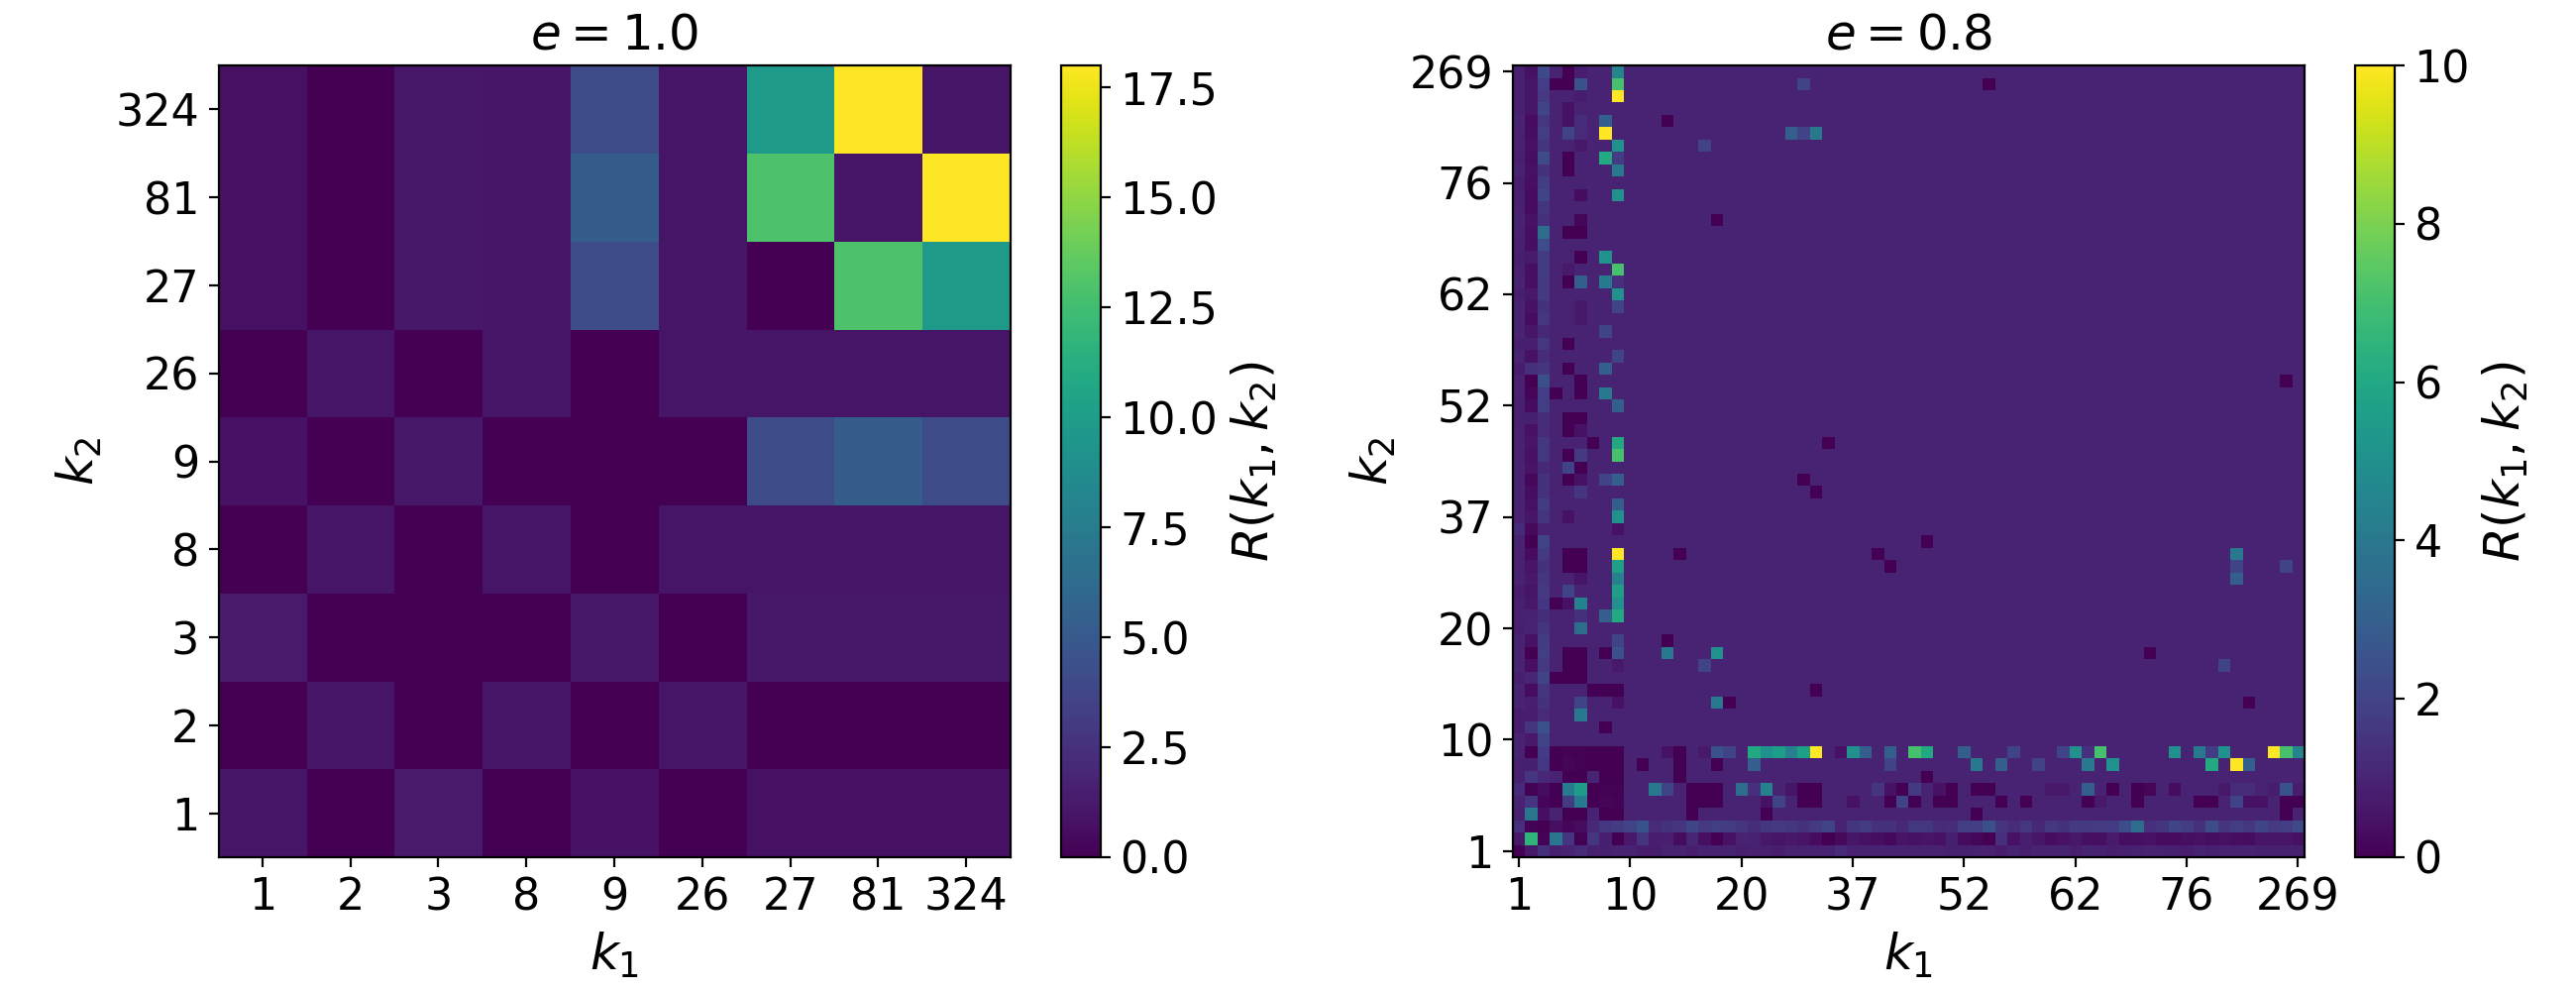
\includegraphics[scale=0.47]{./images/task_6/R_k1_k2_comparison.png} 
	\end{center}
	\caption{Caption.\\} 
	\label{fig:R_k1_k2_comparison} 
\end{figure}

\begin{figure}[!h]
	\begin{center}
	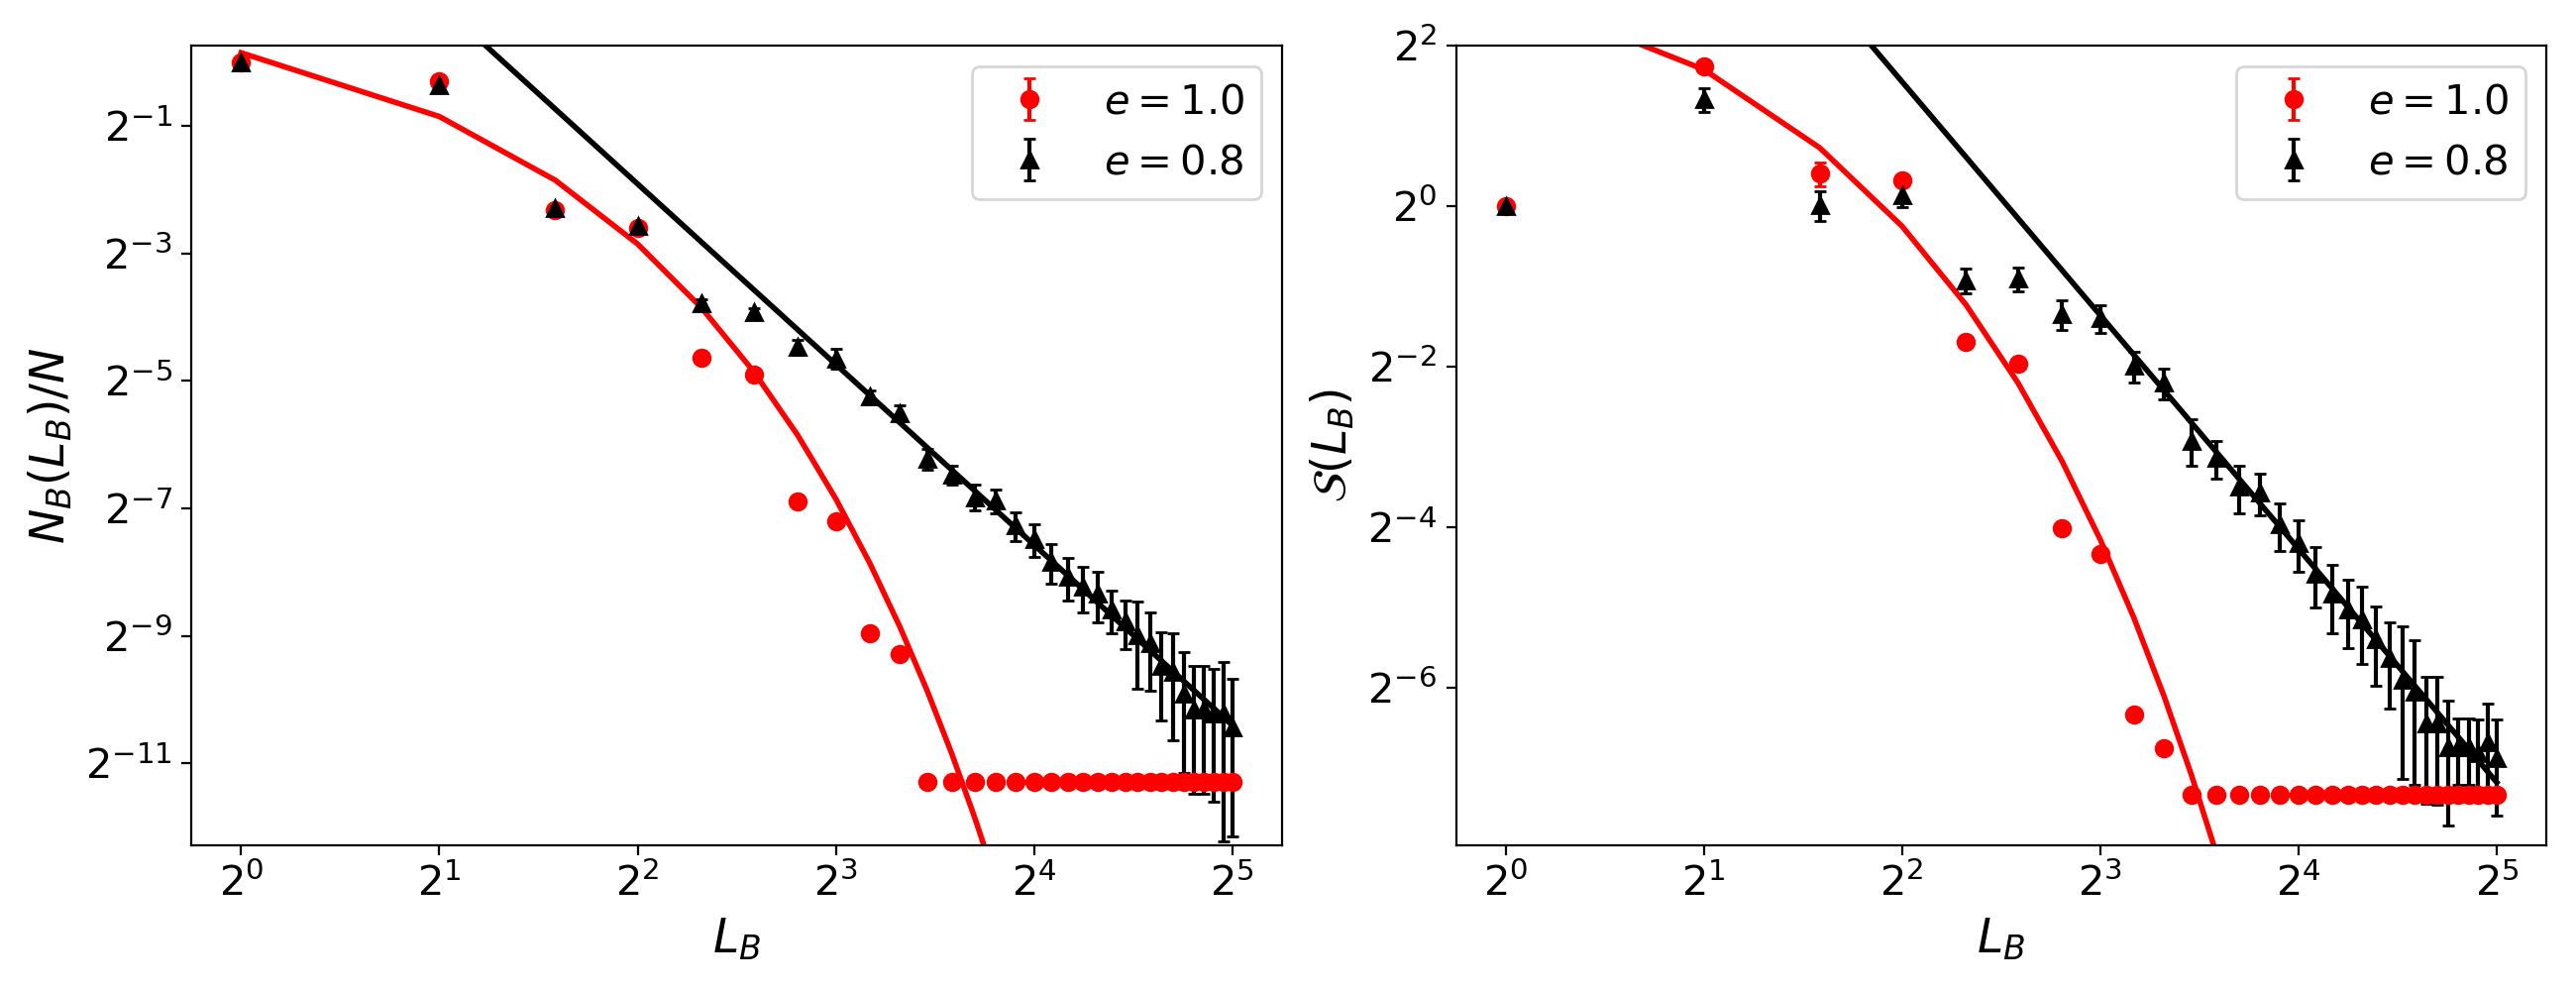
\includegraphics[scale=0.47]{./images/task_6/N_B_and_S_vs_L_B.png} 
	\end{center}
	\caption{Caption.\\} 
	\label{fig:N_B_and_S_vs_L_B} 
\end{figure}


%\begin{figure}
%\centering     %%% not \center
%\subfigure[Figure A]{\label{fig:a}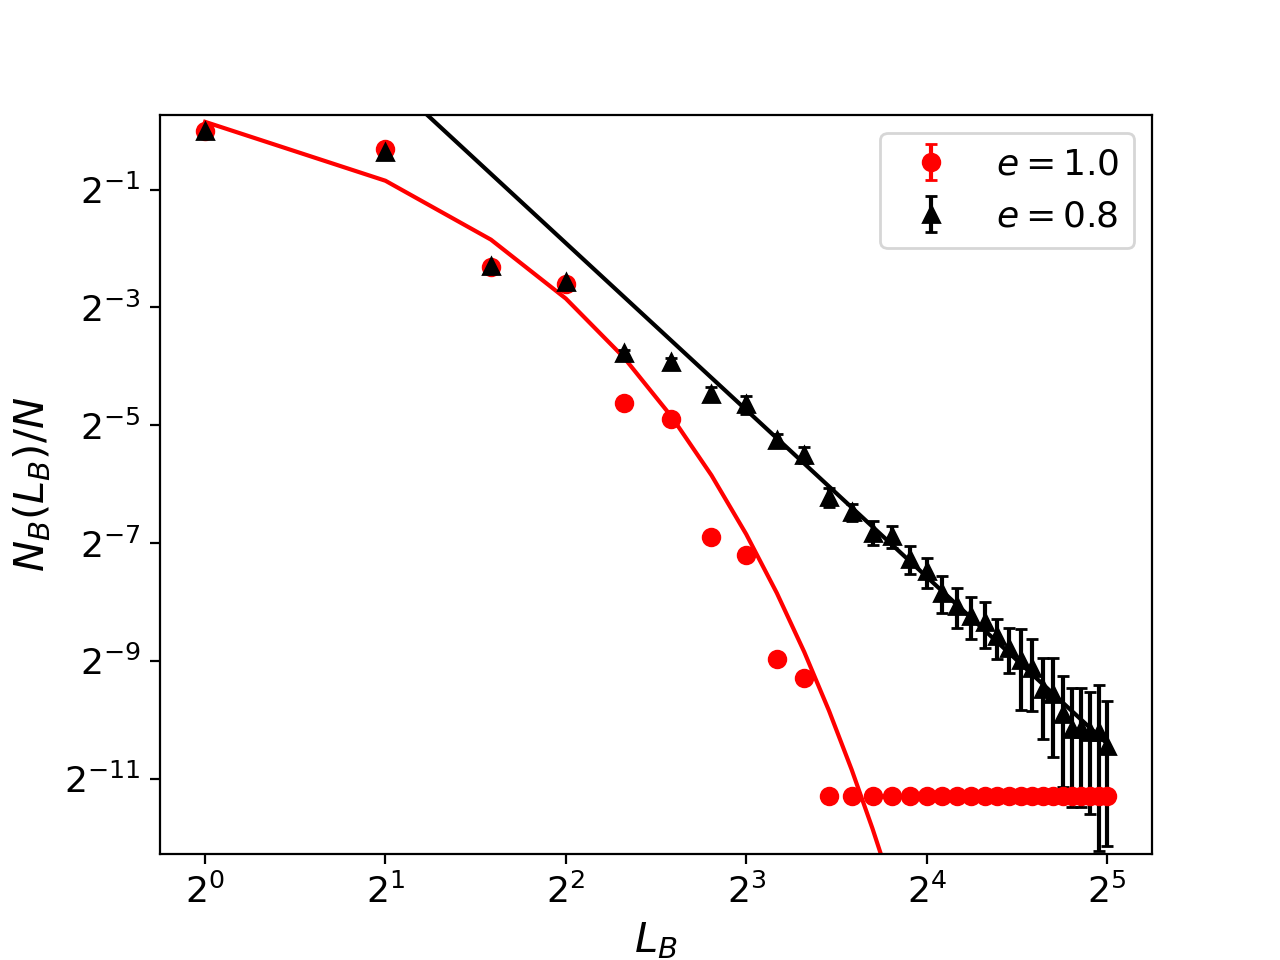
\includegraphics[width=60mm]{./images/task_6/N_B_N_vs_L_B.png}}
%\subfigure[Figure B]{\label{fig:b}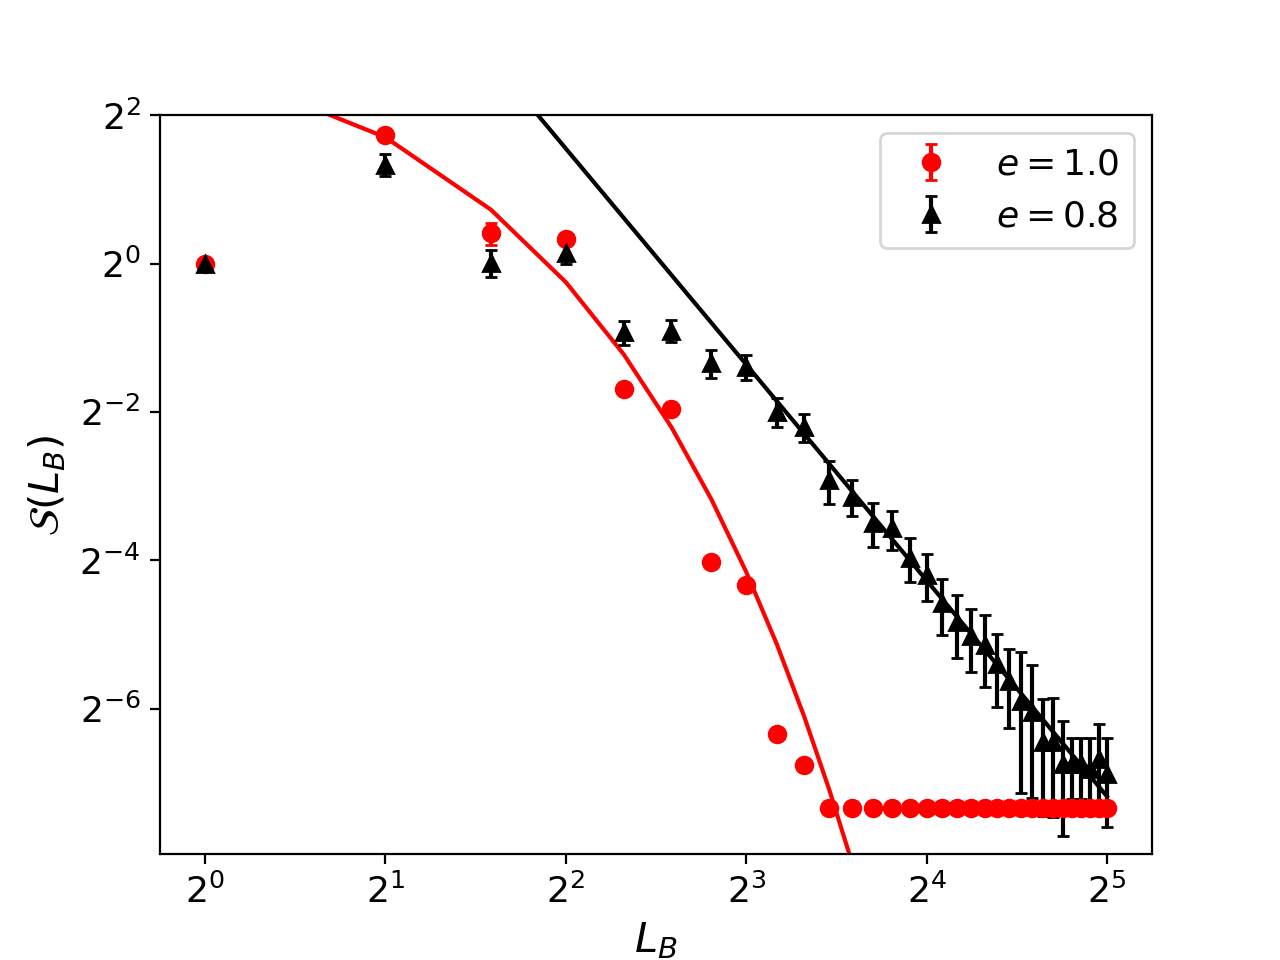
\includegraphics[width=60mm]{./images/task_6/S_vs_L_B.png}}
%\caption{my caption}
%\end{figure}

\lipsum[2-4]


\newpage